% Sequence Integrity Matters — standalone methods paper.
% Source of truth: docs/PAPER_SEQ_INTEGRITY.md (this LaTeX mirrors it).
% Bib: bibliography.bib (shared, reused keys) + seq_integrity_extra.bib (new refs).
% Build: pdflatex seq_integrity && bibtex seq_integrity && pdflatex seq_integrity && pdflatex seq_integrity
\documentclass[conference]{IEEEtran}

\usepackage{amsmath,amssymb,amsfonts}
\usepackage{graphicx}
\usepackage{booktabs}
\usepackage{array}
\usepackage{url}
\usepackage{xcolor}
\usepackage{hyperref}
\hypersetup{colorlinks=true, linkcolor=blue!50!black, citecolor=blue!50!black, urlcolor=blue!50!black,
  pdftitle={Sequence Integrity Matters}, pdfauthor={Hsiu-Chi Tsai}}

\newcommand{\dseq}{\Delta_{\mathrm{seq}}}
\newcommand{\dtraj}{\Delta_{\mathrm{traj}}}
\newcommand{\code}[1]{\texttt{#1}}

\begin{document}
\title{Sequence Integrity Matters: Row-Level Client Partitioning Artifacts in Federated RAN Time-Series Benchmarks}
\author{\IEEEauthorblockN{Hsiu-Chi Tsai}\IEEEauthorblockA{National Yang Ming Chiao Tung University \\ \texttt{nctuie@gmail.com}}}
\maketitle

\begin{abstract}
Federated-learning (FL) benchmarks routinely synthesise client heterogeneity by partitioning a pooled
dataset across clients with a Dirichlet distribution over \emph{rows}. For tabular or image data this is
harmless. For \emph{time series}---where each client subsequently builds sliding windows---it is not:
row-level partitioning scatters a sequence's consecutive timesteps across clients, so the per-client
windows are no longer real trajectories. We show that this \emph{sequence-integrity} violation can
manufacture a striking but spurious finding---that \emph{more} client heterogeneity \emph{improves}
accuracy---in a federated O-RAN slice-SLA benchmark (ColO-RAN), and we dismantle it. The fragmentation
itself is universal (a deterministic consequence of the partition-then-window recipe, confirmed on two
real RAN datasets), but its impact on accuracy is \textbf{task-conditional}: it degrades AUC
substantially only when the prediction target is \emph{sequence-essential} (a small order-invariant
residual remains for window-aggregate targets). We introduce a cheap, partition-free diagnostic,
$\dtraj$---the AUC an intact sequence model gains from temporal \emph{order} over an order-shuffled
baseline---and show the fragmentation AUC gap is a monotone function of it (Spearman $0.95$ across $11$
ColO-RAN targets; Spearman $1.00$ / Pearson $0.99$ in a controlled synthetic study). The artifact is
architecture-invariant for order-using models (LSTM, GRU) and absent for order-blind models, confirming
it is sequence-specific. We give a corrected partitioning protocol (partition by entity/run; synthesise
heterogeneity with \emph{run-level} Dirichlet) and recommend $\dtraj$ as a pre-submission screen. On a
second real dataset (Open RAN Commercial Traffic Twinning) the mechanism replicates but the AUC impact
does not---as the diagnostic predicts for its persistent targets---serving as a negative control.
\end{abstract}

\section{Introduction}
Client heterogeneity (non-IID data) is the defining difficulty of FL, and benchmarks emulate it by
splitting a pooled dataset with a Dirichlet($\alpha$) distribution: small $\alpha$ $\rightarrow$ skewed,
large $\alpha$ $\rightarrow$ near-IID. This recipe is near-universal~\cite{Hsu2019_Dirichlet,
Li2022_NIIDBench,Beutel2020_Flower} and, for i.i.d.-sample data (images, tabular rows), statistically
sound.

Time-series FL inherits the recipe but adds a step: each client turns its rows into fixed-length sliding
windows for a sequence model. Here the recipe quietly breaks. If rows are assigned to clients
independently, a run's consecutive timesteps are \emph{scattered} across clients; when a client then
windows its rows (sorted by time), each ``window'' is a set of non-consecutive snapshots, and the label
attached to it belongs to a temporally mismatched step. The sequence model is trained on temporally
incoherent (window, label) pairs.

We encountered this concretely. In a federated O-RAN slice-SLA prediction benchmark on the
ColO-RAN/Colosseum testbed~\cite{Polese2022}, partitioning by Dirichlet over rows produced an
\emph{inverted} heterogeneity curve: AUC rose as $\alpha$ fell (more skew $\rightarrow$ better accuracy),
the opposite of the FL norm---recent large-scale assessments find heterogeneity \emph{harms}
accuracy~\cite{JimenezGutierrez2025_NonIID}. The tempting reading---that RAN telemetry has special
cell-conditional structure---does not survive controls. A \textbf{run-level} Dirichlet (whole runs
assigned with the same skew) recovers the natural-partition accuracy and erases the inversion; breaking
entity coherence while keeping runs intact costs ${\sim}0$ AUC. The apparent inversion is a
\textbf{sequence-integrity artifact of how the non-IID partition is constructed}, not a property of the
data.

\textbf{Contributions.} (1) We identify and characterise the \emph{sequence-integrity pitfall} of
row-level partitioning in time-series FL benchmarks, with a simple \emph{fragmentation audit metric}.
(2) We show the AUC impact is \textbf{task-conditional} and introduce $\dseq$/$\dtraj$, capacity-matched,
partition-free diagnostics that \emph{predict} the gap. (3) We give the mechanism (run-rate vs.\
trajectory; order vs.\ consecutiveness) and a careful theory: the diagnostic is monotone, \emph{not} a
bound (the natural $\text{gap}\le\dseq$ conjecture is falsified). (4) We establish architecture-invariance
(LSTM, GRU) and order-blind sanity controls. (5) We give a corrected protocol and a negative control on a
second real RAN dataset.

\section{Related Work}
\textbf{(a) The Dirichlet partitioning convention.} Simulating non-IID clients by a Dirichlet
distribution over labels/rows is the de-facto FL-benchmark standard---codified by
NIID-Bench~\cite{Li2022_NIIDBench} and shipped as the default partitioner in FL
frameworks~\cite{Beutel2020_Flower}. It is sound for \emph{i.i.d.-sample} data; our point is that
time-series FL \emph{inherits} it and then adds per-client windowing, where it silently breaks. The
``more heterogeneity helps'' reading we dismantle is especially suspect because the established norm is
the opposite---heterogeneity \emph{harms}~\cite{JimenezGutierrez2025_NonIID}---so an \emph{inverted} curve
should itself be a red flag for an artifact.

\textbf{(b) Windowing leakage in time series.} A known pitfall is generating windows \emph{before} the
train/test split, leaking future context into training~\cite{HiddenLeaks2025}. This is \emph{a different
failure mode}: centralized train/test causality (it inflates scores), not federated client partitioning.
Ours is within-training, federated-specific, and \emph{degrades}---about per-client window integrity
across clients.

\textbf{(b$'$) Temporal-order ablation (our $\dtraj$ method has precedent).} Shuffling timesteps to probe
a model's reliance on temporal order is established---temporal-order verification~\cite{Misra2016_ShuffleLearn}
and segment-shuffle representation learning~\cite{Grover2024_S3}, which notes non-adjacent timesteps can
carry strong dependencies. We do \emph{not} claim the shuffle ablation as novel; we reuse it for a new
purpose---predicting/screening the federated fragmentation gap---and show (Sec.~\ref{sec:hunt}) that the
shuffle destroys \emph{order} whereas row-level fragmentation destroys \emph{consecutiveness}.

\textbf{(c) Temporal fragmentation as a deployment challenge.} Some FL works note local time-series can be
``fragmented'' and that this degrades feature extraction. We differ: the fragmentation here is
\emph{manufactured by the row-level recipe as a benchmark artifact}, is \emph{task-conditional} with a
\emph{predictive diagnostic}, and can produce a \emph{qualitatively false finding}.
FedSL~\cite{Abedi2020_FedSL} instead studies legitimately sequentially-split sequences---a different
setting.

\textbf{(d) FL time-series / RAN benchmarks.} FL traffic/throughput
forecasting~\cite{Pavlidis2024_FLMobile,Perifanis2023_5GTraffic,arXiv2508_08479}, O-RAN
toolchains~\cite{OpenRANGym2022,Polese2022,Twinning2024_dataset}, and FL forecasting
benchmarks~\cite{Hallak2025_FLForget} are the landscape. Susceptibility hinges on the partition-then-window
order (Sec.~\ref{sec:protocol}): entity-partitioned benchmarks are safe; row-Dirichlet ones are at risk.

\section{The Sequence-Integrity Pitfall}\label{sec:pitfall}
A pooled series is split into clients, then each client builds length-$L$ sliding windows within its rows
(sorted by step). \emph{Intact} partitions (natural entity, or run-level Dirichlet) keep whole groups
together $\rightarrow$ genuine trajectories. \emph{Row-level} partitions scatter a group's rows
$\rightarrow$ fragmented windows.

\textbf{Audit metric.} The fragmentation score = fraction of per-client windows with contiguous
\code{step\_idx}: $1.0$ for intact, ${\sim}0$ for row-level on both datasets we study.

\begin{table}[t]\centering\caption{Fragmentation audit (fraction of contiguous windows).}\label{tab:audit}
\begin{tabular}{lrrr}\toprule
dataset & intact & random\_split & dirichlet \\\midrule
ColO-RAN & $1.000$ & ${\sim}0$ & ${\sim}0$ \\
Twinning & $1.0000$ & $0.0002$ & $0.0031$ \\\bottomrule
\end{tabular}\end{table}

The audit is \emph{necessary but not sufficient} for an AUC impact---a window can be fragmented yet the
task unharmed (Sec.~\ref{sec:diag}). Fragmentation alters within-window \emph{order}, \emph{which} steps
populate a window, and the window-to-label \emph{alignment}.

\section{The $\dseq$ / $\dtraj$ Diagnostic and Mechanism}\label{sec:diag}
\textbf{Diagnostics (capacity-matched, partition-free).} $\dseq = \mathrm{AUC}(\text{seq LSTM}) -
\mathrm{AUC}(\text{same LSTM, length-1 window})$: value of the multi-step window over a single step.
$\dtraj = \mathrm{AUC}(\text{seq LSTM}) - \mathrm{AUC}(\text{same LSTM, order-shuffled windows})$:
isolates the \emph{order/trajectory} value (the partition-vulnerable part); the cleaner predictor.

\textbf{Gap decomposition.} The gap splits into (i) a \emph{trajectory component} (only sequence models;
$\propto\dtraj$; dominant for white-noise targets) and (ii) a small \emph{window-content component} (any
model, only for \emph{aggregate} targets). A no-sequence mean-pool MLP isolates (ii): $0.000$ for a point
target, a real $0.025$ for a $5$-step-smoothed target ($\ll$ the LSTM's $0.082$).

\textbf{Mechanism: run-rate vs.\ trajectory.} A target's predictability splits into a partition-invariant
\emph{run-rate} (estimable order-free from any sample) and a partition-vulnerable \emph{trajectory}. The
source's lag-1 autocorrelation is a pre-diagnostic (Table~\ref{tab:autocorr}).

\begin{table}[t]\centering\caption{Source-column lag-1 autocorrelation (ColO-RAN).}\label{tab:autocorr}
\begin{tabular}{lrcc}\toprule
source & autocorr & nature & $\dtraj$/gap \\\midrule
tx\_brate\_dl & $0.984$ & run-rate & ${\sim}0$ \\
dl\_buffer & $0.999$ & run-rate & ${\sim}0$ \\
dl\_mcs & $0.902$ & run-rate & ${\sim}0$ \\
dl\_cqi & $0.553$ & moderate & ${\sim}0$ \\
\textbf{ul\_bler} & $\mathbf{0.022}$ & \textbf{trajectory} & $\mathbf{0.22/0.15}$ \\\bottomrule
\end{tabular}\end{table}

\textbf{A diagnostic, not a bound.} The gap is monotone in $\dtraj$ but we do \emph{not} claim a bound.
The conjecture $\text{gap}\le\dseq$ is \emph{falsified}: with a pure-trajectory synthetic target,
fragmented training is mis-led below the single-step ceiling ($\text{gap}>\dseq$), whereas real BLER
(with a run-rate fallback) gives $\text{gap}<\dseq$.

\section{Experiments}
\textbf{5.1 Synthetic causal control.} Multivariate AR runs; a knob $\lambda$ interpolates a target between
instantaneous and trajectory dependence; pos-rate held ${\sim}0.5$, all else fixed. The gap is monotone in
$\dseq$ (Pearson $0.986$) and the $\text{gap}\le\dseq$ bound is falsified at high $\lambda$.

\textbf{5.2 ColO-RAN $\dseq$ law (main result).} $11$ targets, $5$ seeds, OOD-by-tr split
(Table~\ref{tab:law}). The gap is monotone in $\dseq$ (Pearson $0.943$, Spearman $0.918$, OLS slope CI95
$[0.706,1.113]$ excludes $0$) and cleaner in $\dtraj$ (Pearson $0.974$, Spearman $0.945$). BLER targets:
gap $0.08$--$0.16$ ($5$-seed paired-bootstrap CIs exclude $0$); CQI/MCS/buffer/throughput: gap ${\sim}0$.
\code{bler\_th10} reproduces the established ColO-RAN gap (intact $0.908$ / row $0.757$). The law and
its $\dtraj$ refinement are shown in Fig.~\ref{fig:law}.

\begin{figure*}[t]\centering
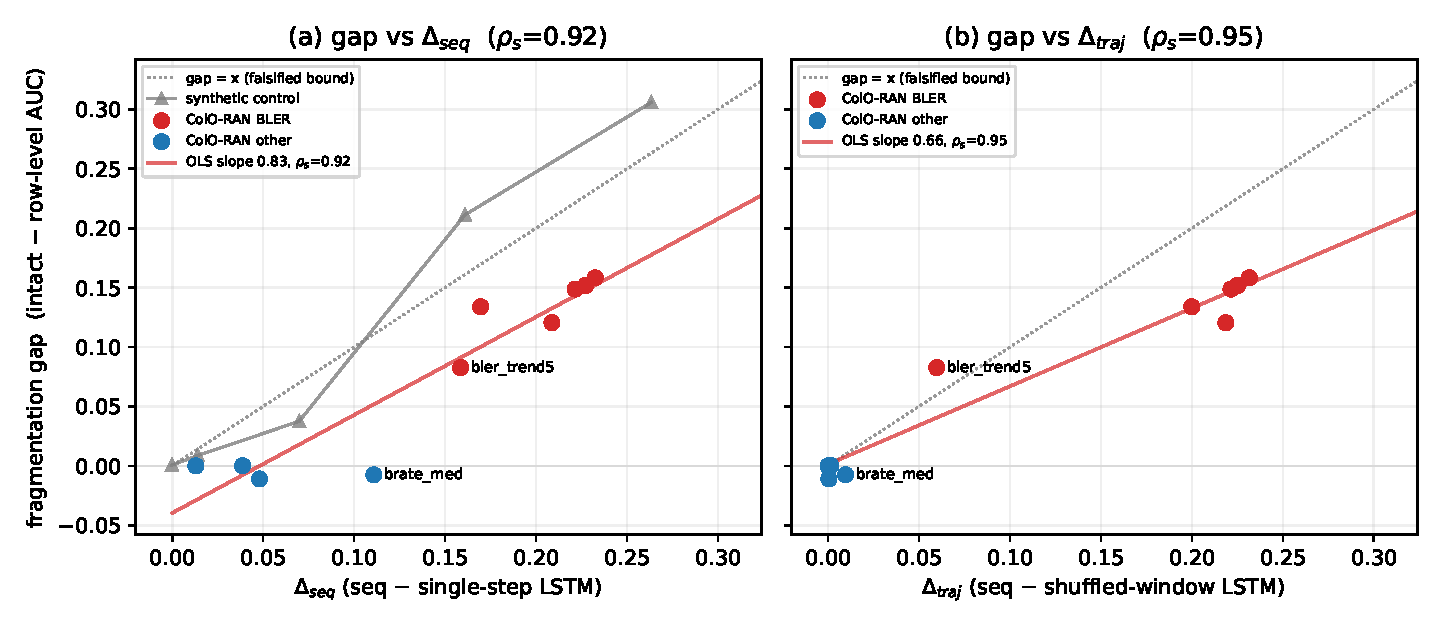
\includegraphics[width=0.92\textwidth]{../artifacts/figures/seq_integrity_law.pdf}
\caption{The fragmentation AUC gap (intact $-$ row-level) is a monotone function of the
sequence-essentiality diagnostic. \textbf{(a)} vs.\ $\dseq$ (seq $-$ single-step LSTM), with the
synthetic controlled backbone and the $\text{gap}=x$ line (the \emph{falsified} bound). \textbf{(b)} vs.\
the order-isolating $\dtraj$ (seq $-$ shuffled-window LSTM): tighter ($\rho_s{=}0.95$) and pulls the
persistent \code{brate\_med} deviator onto the origin. Order-free targets (CQI/MCS/buffer/throughput)
cluster at $\text{gap}{\approx}0$; BLER targets rise with the diagnostic. Slopes $<1$ in (b) reflect
$\dtraj \ge \text{gap}$ (it over-predicts; Sec.~\ref{sec:hunt}).}\label{fig:law}
\end{figure*}

\begin{table}[t]\centering\caption{ColO-RAN $\dseq$ law (11 targets).}\label{tab:law}
\begin{tabular}{lrrr}\toprule
target & $\dseq$ & $\dtraj$ & gap \\\midrule
buffer\_med & $0.013$ & $0.000$ & $+0.000$ \\
mcs\_med & $0.039$ & $0.002$ & $+0.000$ \\
cqi\_med & $0.048$ & $0.001$ & $-0.011$ \\
brate\_med & $0.111$ & $0.010$ & $-0.008$ \\
bler\_trend5 & $0.159$ & $0.060$ & $+0.083$ \\
bler\_k2 & $0.170$ & $0.200$ & $+0.134$ \\
bler\_k3 & $0.209$ & $0.219$ & $+0.121$ \\
bler\_th20 & $0.221$ & $0.222$ & $+0.149$ \\
bler\_th10 & $0.227$ & $0.225$ & $+0.152$ \\
bler\_th05 & $0.227$ & $0.225$ & $+0.152$ \\
bler\_k5 & $0.233$ & $0.232$ & $+0.158$ \\\bottomrule
\end{tabular}\end{table}

\textbf{5.3 Architecture invariance + sanity.} A no-sequence mean-pool MLP shows gap ${\sim}0$ even for
high-$\dseq$ BLER (max $0.025$, an order below the LSTM's $0.16$) $\rightarrow$ the gap is
sequence-specific. LSTM and GRU both learn the BLER trajectory (intact ${\approx}0.90$) and show the gap
tracking $\dseq$. Our small Transformer has no positional encoding, so self-attention with mean-pooling is
permutation-invariant---it is \emph{order-blind by construction} (intact BLER $0.69 \approx$ MLP $0.66$)
and acts as a second no-sequence sanity: both order-blind models show a negligible BLER gap (MLP $+0.0001$,
Transformer $+0.006$), an order of magnitude below the order-using LSTM/GRU ($+0.16$/$+0.15$). A
positional-encoded Transformer is untested (attention's permutation-invariance impeding order modeling is
a known limitation).

\textbf{5.4 Twinning negative control + hunt.}\label{sec:hunt} On Open RAN Commercial Traffic
Twinning~\cite{Twinning2024_dataset} (entity = UE; real Madrid LTE traffic twinned via Colosseum), the
mechanism replicates (audit intact $1.0$ vs.\ row ${\sim}0$, $6858$ (run,UE) groups, $31$M rows) but the
AUC impact does not (next-step CQI/MCS gap ${\sim}0$). A hunt for a \emph{within-Twinning}
sequence-essential positive (drop-event targets) found targets that are $\dtraj$-positive ($0.07$--$0.13$)
yet show no gap ($+0.002$): row-level windowing keeps each window sorted-ascending (only gappy), so it
\textbf{preserves order and destroys only consecutiveness} (the row AUC tracks the ordered seqC, not the
shuffled baseline), and a drop-event needs order but tolerates gaps. So $\dtraj \ge \text{gap}$
empirically; it conflates order with consecutiveness. Even Twinning's sequence-essential targets are
fragmentation-robust.

\section{A Correct Partitioning Protocol}\label{sec:protocol}
(1) Partition by natural \emph{entity/run} (each holds its intact stream). (2) To synthesise
heterogeneity, use \textbf{run-level Dirichlet} (whole runs, skewed assignment), never row-level. (3)
Pre-screen with $\dtraj$, then \emph{confirm with the run-level-vs-row-level control}: a $\dtraj\approx0$
benchmark is safe; a large $\dtraj$ flags a benchmark to investigate, but $\dtraj$ can over-predict (it
destroys the last-step/order signal that END-aligned fragmentation preserves), so the partition control is
the decisive test.

A spot-audit of representative FL-TS benchmarks (Table~\ref{tab:atrisk}; we classify the stated recipe---a
definitive verdict needs each paper's code) shows well-designed \emph{domain} benchmarks predominantly
partition by \emph{entity} (safe); the risk is transplanting the generic image/tabular Dirichlet-over-rows
convention onto a pooled time series. The partition-then-window \emph{order is rarely reported}, so
susceptibility often cannot be determined from the text---itself the finding motivating our reporting
recommendation. We do not assert any prior benchmark is flawed.

\begin{table}[t]\centering\caption{Spot-audit by stated partition recipe.}\label{tab:atrisk}
\begin{tabular}{p{3.0cm}p{1.95cm}p{2.25cm}}\toprule
benchmark & stated partition & susceptibility \\\midrule
Beijing air-quality FL~\cite{Hallak2025_FLForget} & entity (per station), windows post-partition & safe \\
Mobile-net traffic FL~\cite{Pavlidis2024_FLMobile} & entity (per BS) & safe \\
5G BS traffic~\cite{Perifanis2023_5GTraffic} & entity (per BS) & safe \\
NIID-Bench / ProFed~\cite{Li2022_NIIDBench,ProFed2025} & Dirichlet over rows (image/tabular) & convention's home; unsafe if transplanted to a pooled TS \\
ColO-RAN \code{fl\_v7} (this work) & Dirichlet over rows of a pooled series & at-risk (manufactured the inverted-$\alpha$ artifact) \\\bottomrule
\end{tabular}\end{table}

\section{Limitations and Threats to Validity}
The $\dseq$/$\dtraj$ law is an \emph{empirical} monotone diagnostic, not a proven bound (synthetic
super-linearity vs.\ real sub-linearity shows the constant is data-dependent). $\dtraj$ \emph{over-predicts}
for order-but-gap-robust targets (Sec.~\ref{sec:hunt}); it is a cheap screen, and the
run-level-vs-row-level control is ground truth. Architecture coverage is LSTM + GRU (order-using) plus a
mean-pool MLP and a no-positional-encoding Transformer (both order-blind sanities); a positional-encoded
Transformer is untested. The Twinning AUC-impact null is a $1$-seed smoke; ColO-RAN gaps use $5$-seed
paired bootstrap ($n{=}5$). \code{ul\_sinr} was dropped pre-results (degenerate: median at a mass point
$\rightarrow$ undefined AUC). Partition client counts differ by mode (iid $=7$ BS; Dirichlet $=8$),
immaterial to the global-test gap.

\section{Conclusion}
Row-level Dirichlet partitioning---a near-universal FL-benchmark convention---can manufacture spurious
findings in time-series FL by fragmenting per-client windows. The pitfall is real but
\emph{task-conditional}: it bites sequence-essential tasks (large $\dtraj$) and spares order-free ones,
which is why it has gone unnoticed. We provide the audit metric, the $\dtraj$ diagnostic, the mechanism,
and a corrected protocol. We urge time-series FL benchmarks to partition by entity/run (or run-level
Dirichlet) and to report $\dtraj$ and the partition-then-window order.

\section*{Reproducibility}
Pre-registration, results, theory, and scripts (synthetic; ColO-RAN sweep; $\dtraj$ addendum;
architecture invariance; Twinning audit + AUC-impact + hunt; \code{window\_cache} with a bit-exact test)
are in the project repository. All runs: local RTX 4060 Ti (memory-caged) + a V100 ColO-RAN sweep.

\bibliographystyle{IEEEtran}
\bibliography{bibliography,seq_integrity_extra}
\end{document}
